\section{Lezione del 27-28/04/2018}

\subsection{Red-Black Trees}

I \emph{Red-Black Trees} sono ABR i cui nodi hanno un campo \emph{colore} $x.col$, che può essere:
\begin{itemize}[noitemsep]
    \item \textbf{R} per il rosso;
    \item \textbf{B} per il nero.
\end{itemize}

\paragraph{Accorgimento} $\const{nil}$ sarà in realtà un nodo,
$T.nil$, con $T.nil.col = B$.

\paragraph{Caratteristiche} \emph{RB-tree} è in realtà un ABR tale che:
\begin{enumerate}[label=($\arabic*$)]
    \item Ogni nodo $x$ ha $x.col \in \{R,B\}$; \label{rbtree:1}
    \item La radice $root$ ha $root.col = B$; \label{rbtree:2}
    \item Le foglie ($T.nil$) sono $B$; \label{rbtree:3}
    \item Se $x$ è $R$, i figli sono $B$; \label{rbtree:4}
    \item Per ogni nodo $x$, ogni cammino da $x$ a una qualsiasi delle foglie
    ha lo stesso numero di nodi $B$ (calcolato con $bh(x)$). \label{rbtree:5}
\end{enumerate} 

\begin{figure}[hbt]
    \centering
    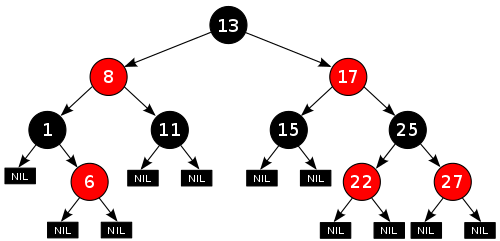
\includegraphics[width=\textwidth]{img/rb-tree-ex.png}
    \caption{Esempio di un RB-tree.}
\end{figure}
\pagebreak

È possibile notare che: 
\begin{itemize}
    \item In caso non ci fossero nodi rossi, avremo un albero
    perfettamente bilanciato;
    \item In ogni cammino, il \verb|#| di nodi \textbf{B} è almeno la
    metà del \verb|#| dei nodi \textbf{R}
\end{itemize}

\paragraph{Osservazione} Se $T$ è un \emph{RB-tree} con $n$ nodi interni ($\neq \const{nil}$)
e $h$ altezza, allora vale
$$h \leq 2 \log (n + 1)$$

\subparagraph{Dimostrazione} Consideriamo 
$$n_x \geq 2^{bh(x)} - 1$$
La dimostrazione è per induzione su $h_x$ (altezza del sotto-albero radicato in $x$).

\begin{description}
    \item[$(h_x = 1)$] Allora ho solo 
    $T.nil \Rightarrow n_x = 0 = 2^0 - 1 \qquad (2^0 \text{ con } 0 = bh(x))$
    \item[$(h_x > 1)$] Consideriamo $x$ radice. $x$ ha due figli, $x_1$ e $x_2$.\par
    Sicuramente vale $h_1,h_2 < h$. Per ipotesi induttiva, valgono:
    $$n_{x_1} \geq 2^{bh(x_1)} - 1$$
    $$n_{x_2} \geq 2^{bh(x_2)} - 1$$
    \begin{align*}
        n_x & = n_{x_1} + n_{x_2} + 1 \\
        & \geq 2^{bh(x_1)} + 2^{bh(x_2)} - 1 \\
        & \geq 2 \cdot 2^{bh(x)-1} - 1 = 2^{bh(x)} - 1 \\
        & \qquad (\text{valgono } bh(x_1) \geq bh(x)-1, \ bh(x_2) \geq bh(x)-1) \\
        \text{Comples}&\text{sivamente}\\
        n & = n_{root} \geq 2^{bh(root)} - 1
    \end{align*}
    Essendo $bh(root) \geq \frac{h}{2}$, posso ottenere
    \begin{align*}
        n_{root} & \geq 2^{bh(root)} - 1 \\
        & 2^{\frac{h}{2}} - 1 \\
        \Rightarrow \ & 2^{\frac{h}{2}} \leq n + 1 \\
        & \frac{h}{2} \leq \log_2(n+1) \Rightarrow h \leq 2 \log_2(n+1) 
    \end{align*}
\end{description}

\subsubsection{Complessità algoritmi RB-Trees}
\texttt{Search, Succ, Min, Pred, Max} hanno un costo di $O(h) = O(\log n)$

%2/5/2018

\subsubsection{RB-Insert e RB-Delete}
A differenza di quelle citate precedentemente, che risultano semplici
sia come complessità asintotica che come implementazione, Bisogna porre 
particolare attenzione a queste due procedure: \texttt{RB-Insert} e \texttt{RB-Delete}.

Per ovviare a ciò, posso utilizzare le \emph{rotazioni}. Consideriamo il seguente albero,
in cui $x$ e $y$ sono nodi normali, mentre $\alpha, \ \beta$ e $\gamma$ sono sotto-alberi
(il colore dei nodi non ha importanza ai fini della procedura che andremo a 
vedere)\footnote{Di conseguenza, applicandola a un \emph{RB-tree}, gli assiomi di validità potrebbero venire violati.}:
\begin{center}
	\begin{tikzpicture}
	\Tree
	[.$x$     
		[.$\alpha$
		]
		[.$y$ 
            [.$\beta$ 
                \edge[blank]; \node[blank]{};
                \edge[blank]; \node[blank]{};
            ]
			[.$\gamma$ 
                \edge[blank]; \node[blank]{};
                \edge[blank]; \node[blank]{};
            ]
		]
	]
	\end{tikzpicture}
\end{center}
Applichiamo la procedura \texttt{Left(T,x)}, ottenendo:
\begin{center}
	\begin{tikzpicture}
	\Tree
	[.$y$
        [.$x$
            [.$\alpha$ 
                \edge[blank]; \node[blank]{};
                \edge[blank]; \node[blank]{};
            ]
            [.$\beta$ 
                \edge[blank]; \node[blank]{};
                \edge[blank]; \node[blank]{};
            ]
		]
		[.$\gamma$ ]
	]
	\end{tikzpicture}
\end{center}

\paragraph{Osservazione} La \emph{visita simmetrica} è identica per i due alberi:
$$\alpha \rightarrow x \rightarrow \beta \rightarrow y \rightarrow \gamma$$

\begin{codebox}
\Procname{\proc{Left}$(T,x)$}
\li $\attrib{x}{right} \gets \attrib{y}{left}$
\li $\attrib{\attrib{x}{right}}{p} \gets x$
\li $\attrib{y}{left} \gets x$
\li $\attrib{x}{p} \gets y$
\li $\proc{Transplant}(T,x,y)$
\end{codebox}

\paragraph{RB-Insert(T, z)} Voglio inserire $z$ nell'albero $T$.
L'idea è quella di porre $z.col = \const{red}$ poichè meno insidioso\footnote{Andando a modificare il numero di nodi neri, cambia l'altezza nera, e la cosa è difficile da sistemare.}.
\begin{itemize}
    \item Se violo \ref{rbtree:2} $\Rightarrow z.col = \const{black}$;
    \item Se violo \ref{rbtree:4}:
    \begin{itemize}
        \item Risolvo localmente;
        \item Sposto verso l'alto il problema.
    \end{itemize}
\end{itemize}

Abbiamo due \emph{macrocasi}. $z.p$ è figlio sinistro, oppure destro. Noi analizzeremo solo il primo: \textbf{z.p figlio sinistro}.
\begin{center}
	\begin{tikzpicture}
	\Tree
	[.$\boldsymbol{z.p.p}$
        [.$\boldsymbol{\color{red} z.p}$
            [.$\boldsymbol{\color{red} z}$
            ]
		]
		[.$y$ 
        \edge[blank]; \node[blank]{};
        \edge[blank]; \node[blank]{};
        ]
    ]
	\end{tikzpicture}
\end{center}
\clearpage
Abbiamo due possibilità per $y$\footnote{I nodi con testo in rosso sono $\const{red}$, %
quelli in grassetto sono $\const{black}$, e quelli normali possono essere sia rossi che neri.}:
\begin{enumerate}
    \item $y.col = \const{red}$. Ci è sufficiente invertire il colore di $z.p.p$ con quello dei figli.
    \begin{center}
        \begin{tikzpicture}
        \Tree
        [.$\boldsymbol{\color{red} z.p.p}$
            [.$\boldsymbol{z.p}$
                [.$\boldsymbol{\color{red} z}$
                ]
            ]
            [.$\boldsymbol{y}$ 
            \edge[blank]; \node[blank]{};
            \edge[blank]; \node[blank]{};
            ]
        ]
        \end{tikzpicture}
    \end{center}
    In questo modo, risolviamo localmente e rimandiamo il problema in alto.
    \item $y.col = \const{black}$. Possiamo distinguere due sottocasi.
    \begin{enumerate}[label=($2.\arabic*$)]
        \item $z$ figlio destro. \label{rbinsert:2.1}
        \begin{center}
            \begin{tikzpicture}
            \Tree
            [.$\boldsymbol{z.p.p}$
                [.$\boldsymbol{\color{red} z.p}$
                    \edge[blank]; \node[blank]{};
                    [.$\boldsymbol{\color{red} z}$
                    ]
                ]
                [.$\boldsymbol{y}$ 
                \edge[blank]; \node[blank]{};
                \edge[blank]; \node[blank]{};
                ]
            ]
            \end{tikzpicture}
        \end{center}
        Voglio finire nel caso \ref{rbinsert:2.2}. Applico \texttt{Left(T,z.p)}, ottenendo:
        \begin{center}
            \begin{tikzpicture}
            \Tree
            [.$\boldsymbol{z.p.p}$
                [.$\boldsymbol{\color{red} z}$
                    [.$\boldsymbol{\color{red} z.p}$ ]
                    \edge[blank]; \node[blank]{};
                ]
                [.$\boldsymbol{y}$ 
                \edge[blank]; \node[blank]{};
                \edge[blank]; \node[blank]{};
                ]
            ]
            \end{tikzpicture}
        \end{center}

        \item $z$ figlio sinistro. \label{rbinsert:2.2}
        \begin{center}
            \begin{tikzpicture}
            \Tree
            [.$\boldsymbol{z.p.p}$
                [.$\boldsymbol{\color{red} z.p}$
                    [.$\boldsymbol{\color{red} z}$ ]
                    \edge[blank]; \node[blank]{};
                ]
                [.$\boldsymbol{y}$ 
                \edge[blank]; \node[blank]{};
                \edge[blank]; \node[blank]{};
                ]
            ]
            \end{tikzpicture}
        \end{center}
        Scambio i colori di $z.p.p$ con $z.p$, ottenendo:
        \begin{center}
            \begin{tikzpicture}
            \Tree
            [.$\boldsymbol{\color{red} z.p.p}$
                [.$\boldsymbol{z.p}$
                    [.$\boldsymbol{\color{red} z}$ ]
                    \edge[blank]; \node[blank]{};
                ]
                [.$\boldsymbol{y}$ 
                \edge[blank]; \node[blank]{};
                \edge[blank]; \node[blank]{};
                ]
            ]
            \end{tikzpicture}
        \end{center}
        Applico \texttt{Right(T,z.p.p)}\footnote{Analoga di \texttt{Left}.}:
        \begin{center}
            \begin{tikzpicture}
            \Tree
            [.$\boldsymbol{z.p}$
                [.$\boldsymbol{\color{red} z}$ 
                    \edge[blank]; \node[blank]{};
                    \edge[blank]; \node[blank]{};
                ]
                [.$\boldsymbol{\color{red} z.p.p}$ 
                    \edge[blank]; \node[blank]{};
                    [.$\boldsymbol{y}$ ]
                ]
            ]
            \end{tikzpicture}
        \end{center}
    \end{enumerate}
\end{enumerate}

\begin{codebox}
\Procname{\proc{RB-Insert}$(T,z)$}
\li $\proc{Insert}(T,z)$
\li $\attrib{z}{col} \gets \const{red}$
\li $\proc{RB-InsertFix}(T,z)$
\end{codebox}
\begin{codebox}
\Procname{\proc{RB-InsertFix}$(T,z)$}
\li \While $\attrib{\attrib{z}{p}}{col} = \const{red}$
\li \Do
        \If $\attrib{z}{p} = \attrib{\attrib{\attrib{z}{p}}{p}}{left}$
        \Comment Macrocaso $z.p$ figlio sinistro
\li     \Then
            $y \gets \attrib{\attrib{\attrib{z}{p}}{p}}{right}$
\li         \If $\attrib{y}{col} = \const{red}$ \Comment Caso 1
\li         \Then
                $\attrib{\attrib{\attrib{z}{p}}{p}}{col} \gets \const{red}$
\li             $\attrib{\attrib{z}{p}}{col} \gets \const{black}$
\li             $\attrib{y}{col} \gets \const{black}$
\li             $z \gets \attrib{\attrib{z}{p}}{p}$
\li         \Else \Comment Caso 2
\li             \If $z = \attrib{\attrib{z}{p}}{right}$ \Comment Caso \ref{rbinsert:2.1}
\li             \Then
                    $\proc{Left}(T,\attrib{z}{p})$
\li                 $z \gets \attrib{z}{left}$
                \End
\zi             \Comment Caso \ref{rbinsert:2.2}
\li             $\attrib{\attrib{z}{p}}{col} \gets \const{black}$
\li             $\attrib{\attrib{\attrib{z}{p}}{p}}{col} \gets \const{red}$
\li             $\proc{Right}(T,\attrib{\attrib{z}{p}}{p})$
            \End
\li     \Else $\dots$ \Comment Macrocaso $z.p$ figlio destro
        \End
    \End
\li $\attrib{\attrib{T}{root}}{col} \gets \const{black}$
\end{codebox}

\subparagraph{Costo}
$$\frac{h}{2} \cong \frac{\log n}{2} \approx \log n \text{ iterazioni senza rotazioni}
    + \proc{Max} \text{ 2 rotazioni.}$$

\paragraph{RB-Delete(T, z)}
La \texttt{Delete} è ancora più problematica\footnote{Ho deciso di ometterla per non saper come rappresentarla in modo adeguato.%
Darò solo una breve osservazione}. Se $z$ è rosso, non ho nessun problema, poichè l'altezza nera non viene toccata.
Altrimenti, i problemi possono essere diversi (radice rossa, due nodi rossi adiacenti, altezza nera inconsistente, ecc\dots).